\documentclass[11pt]{report}
\usepackage{eso-pic,graphicx}
\usepackage[export]{adjustbox}
\usepackage{url}
\usepackage[top=2cm, bottom=2cm, outer=2cm, inner=2cm]{geometry}
\begin{document}
\AddToShipoutPictureBG*{
\includegraphics[width=\paperwidth,height=\paperheight]{images/bkgrnd}}
\begin{center}
\vspace*{2cm}
\textsf{\begin{Huge}
\textbf{ELP­718 ­ Telecom Software Laboratory \\
1st Semester, 2016-18 \\
Abhishek Mishra\\
05 Oct 2016, 5pm\\
Assignment-10}\\
\end{Huge}}
\vspace*{6cm}

\includegraphics[scale=0.12, center]{images/iitlogo}
\end{center}
\pagebreak
\tableofcontents
\vspace{5cm}
\pagebreak
\section{Introduction}
\vspace*{1cm}
This assignment aims to provide a better understanding of the following topics:\\

\begin{flushleft}
1. \textbf{Python}\\
Python is a widely used high-level, general-purpose, interpreted, dynamic programming language.[24][25] Its design philosophy emphasizes code readability, and its syntax allows programmers to express concepts in fewer lines of code than possible in languages such as C++ or Java.[26][27] The language provides constructs intended to enable writing clear programs on both a small and large scale.[28]

Python supports multiple programming paradigms, including object-oriented, imperative and functional programming or procedural styles. It features a dynamic type system and automatic memory management and has a large and comprehensive standard library.[29]

Python interpreters are available for many operating systems, allowing Python code to run on a wide variety of systems. Using third-party tools, such as Py2exe or Pyinstaller,[30] Python code can be packaged into stand-alone executable programs for some of the most popular operating systems, so Python-based software can be distributed to, and used on, those environments with no need to install a Python interpreter.

CPython, the reference implementation of Python, is free and open-source software and has a community-based development model, as do nearly all of its variant implementations. CPython is managed by the non-profit Python Software Foundation.
\end{flushleft}

\begin{flushleft}
2. \textbf{Kivy}\\
Kivy - Open source Python library for rapid development of applications
that make use of innovative user interfaces, such as multi-touch apps.

\end{flushleft}
\newpage
\section{Problem Statement 1}
	This problem requires us to build a GUI containing a six screen system.\\
	First screen being student/admin login option.\\ 		Second screen being user login system.\\
	Third screen being Student Info Form.\\
	Fourth Screen being Student info display form.
	Fifth Screen being Widget system that enables admin to choose between displaying student info and graph of their marks.
	Sixth screen being graph displayed of Subject vs marks.
	%\begin{figure}[h!]
	%\centering
	%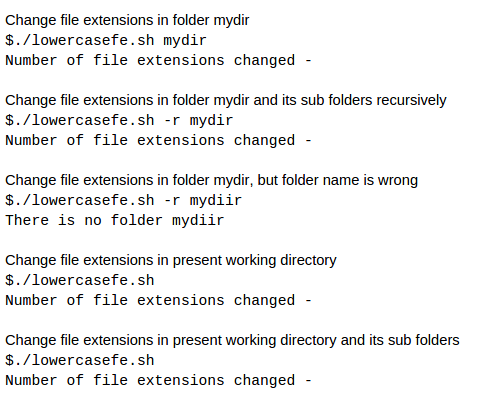
\includegraphics[scale=0.7]{images/Selection_003}	
	%\end{figure}
	\subsection{Assumptions}
	The directory student info isn't formed beforehand and files are also created then only.
	\pagebreak
	\subsection{Structure Chart and Implementation}
	\begin{figure}[h!]
	\centering
	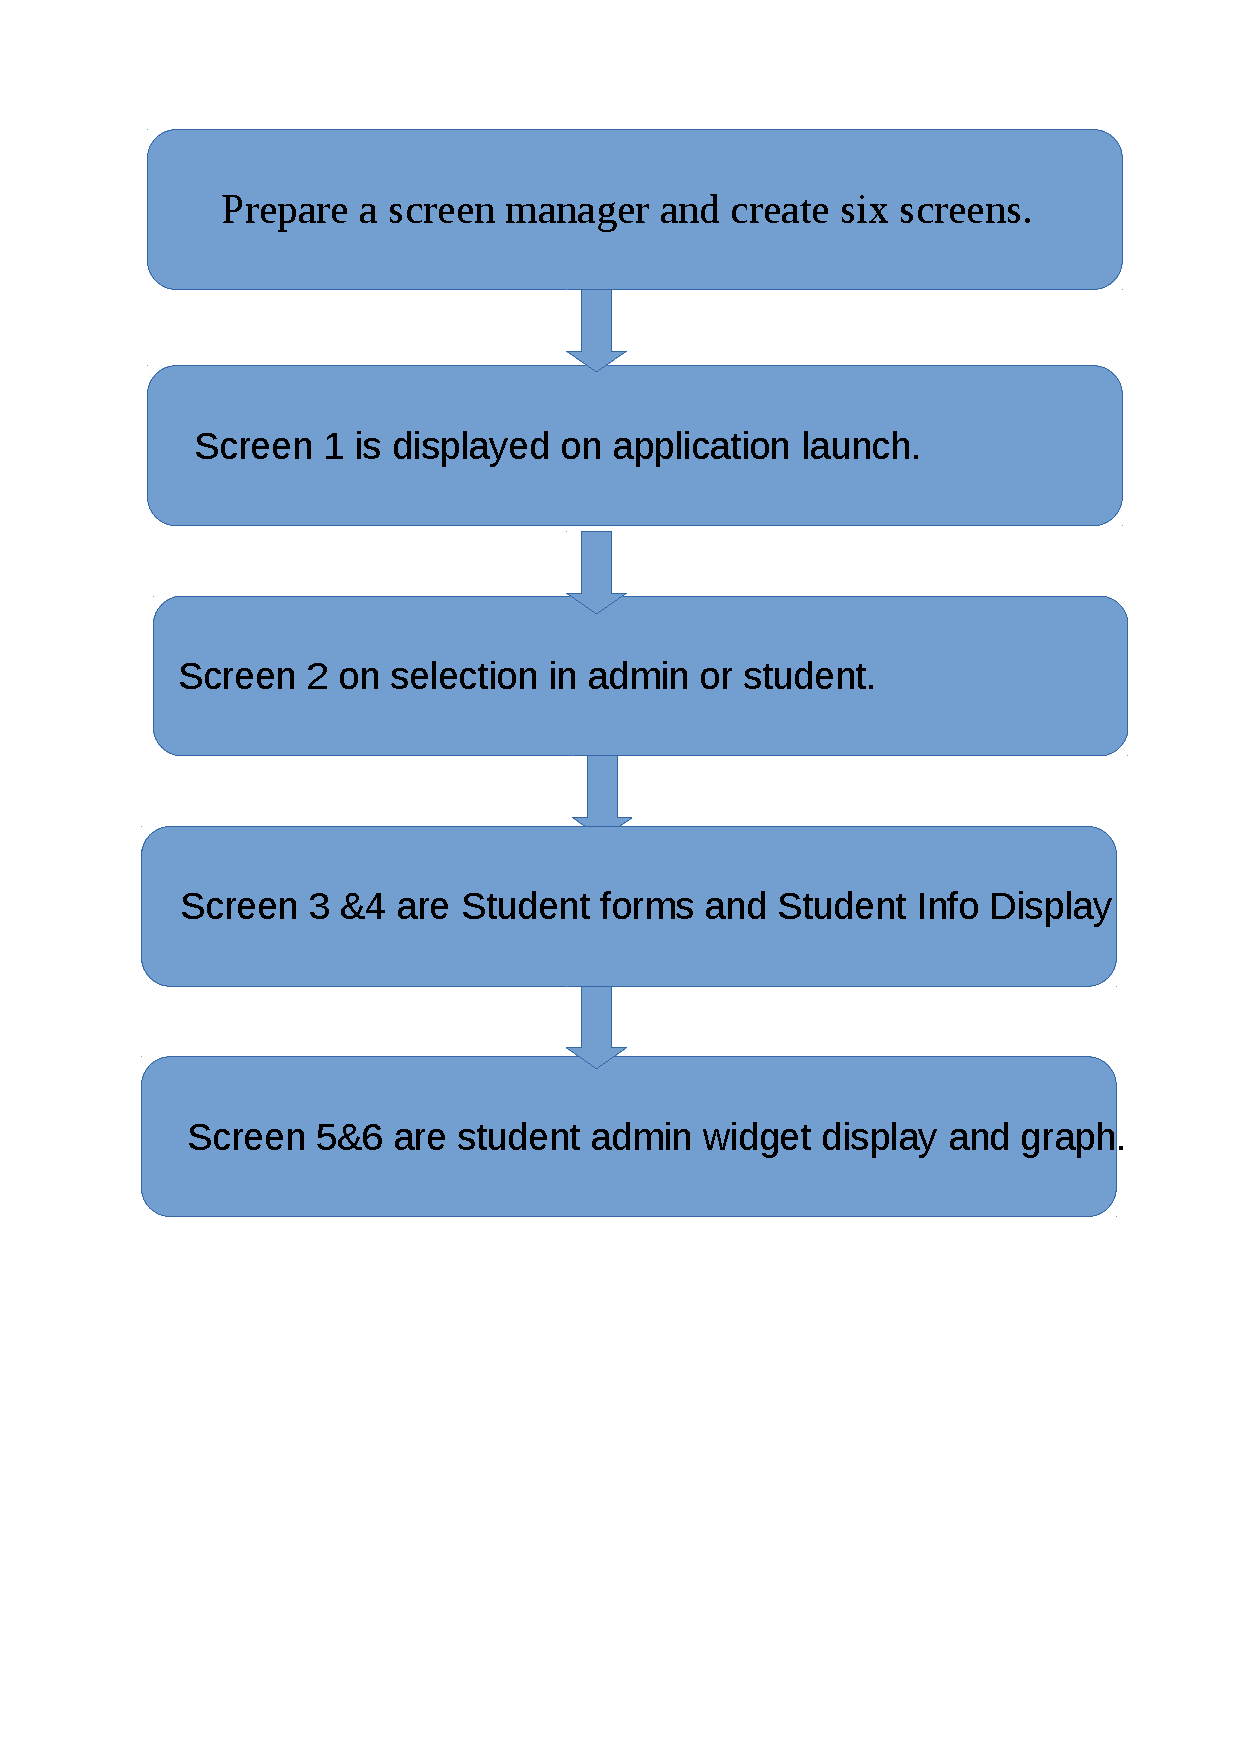
\includegraphics[scale=0.7]{images/shots11}
	\caption{Structure chart for problem 1}
	\end{figure}		
	\pagebreak
	\subsection{Screenshots}
	\begin{figure}[h!]
	\centering
	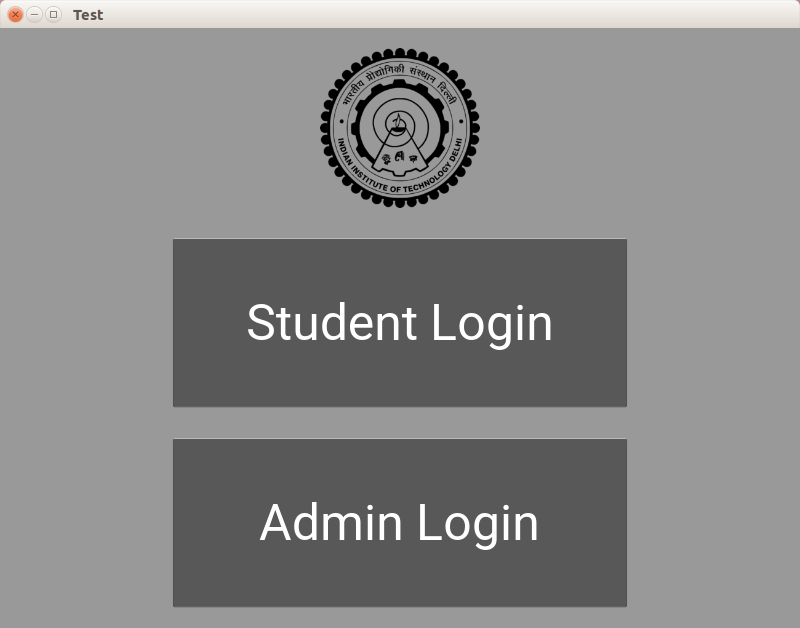
\includegraphics[scale=0.8, center]{images/screenshot1}
	\caption{Screenshot for problem statement 1}
	\end{figure}
	\begin{figure}[h!]
	\centering
	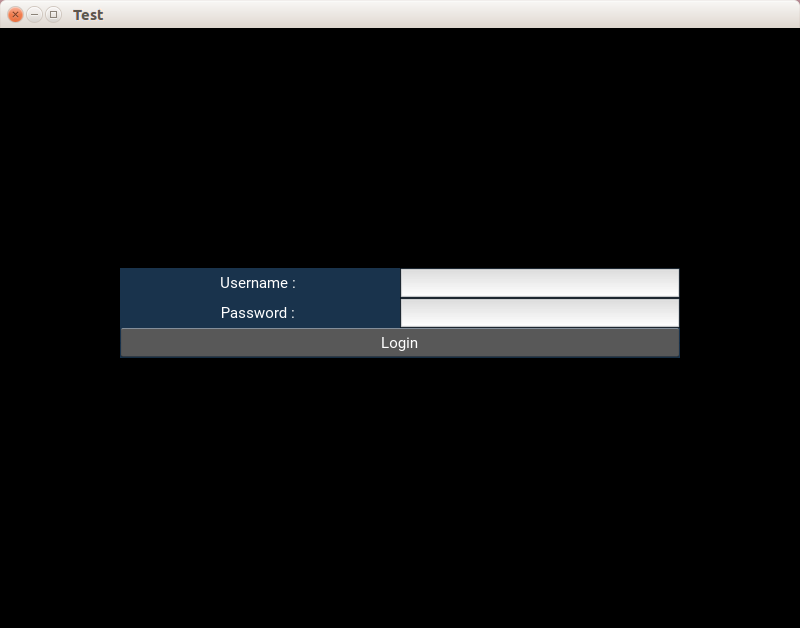
\includegraphics[scale=0.8, center]{images/screenshot2}
	\caption{Screenshot for problem statement 1}
	\end{figure}
	\begin{figure}[h!]
	\centering
	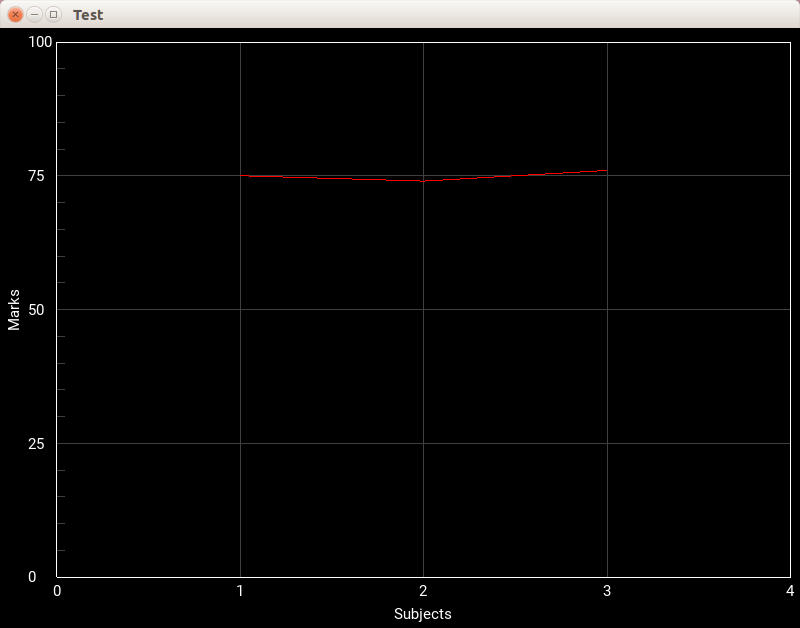
\includegraphics[scale=0.8, center]{images/screenshot3}
	\caption{Screenshot for problem statement 1}
	\end{figure}
	\begin{figure}[h!]
	\centering
	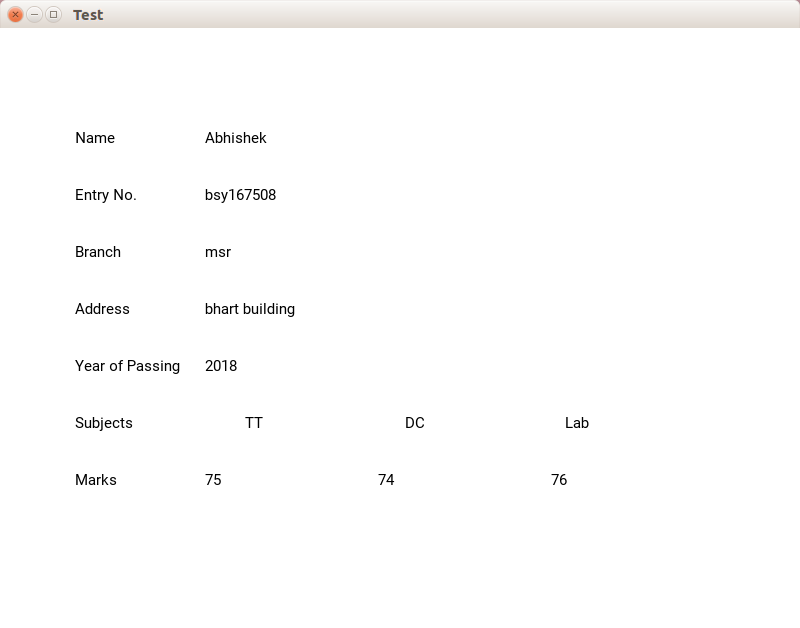
\includegraphics[scale=0.8, center]{images/screenshot4}
	\caption{Screenshot for problem statement 1}
	\end{figure}
	\begin{figure}[h!]
	\centering
	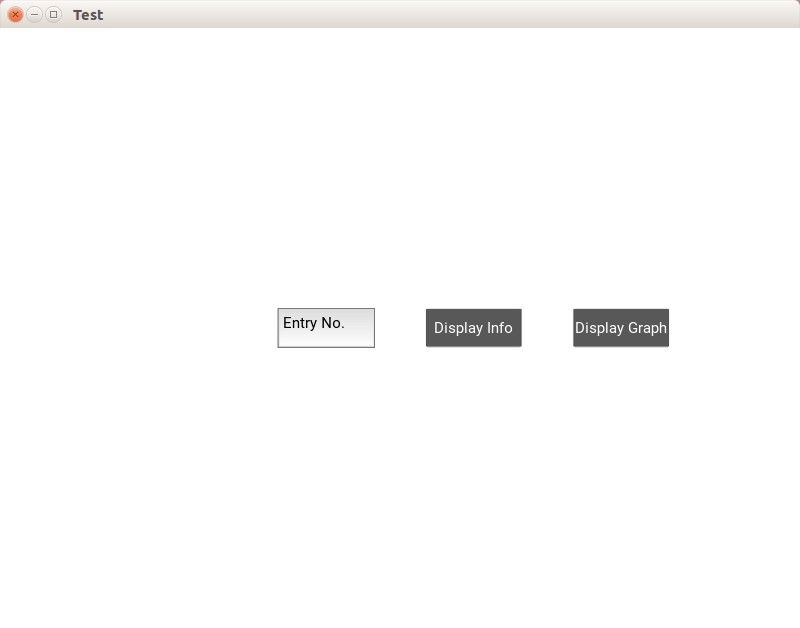
\includegraphics[scale=0.8, center]{images/screenshot5}
	\caption{Screenshot for problem statement 1}
	\end{figure}
	\begin{figure}[h!]
	\centering
	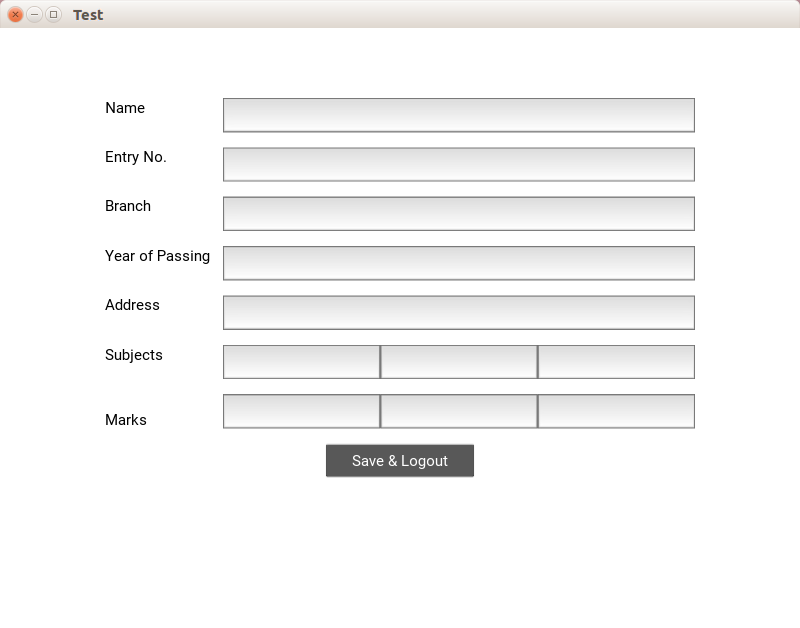
\includegraphics[scale=0.8, center]{images/screenshot6}
	\caption{Screenshot for problem statement 1}
	\end{figure}
	\pagebreak
	\iffalse
\section{Problem Statement 2}
	The problem requires you to display system information in the following manner. \\
	\begin{figure}[h!]
	\centering
	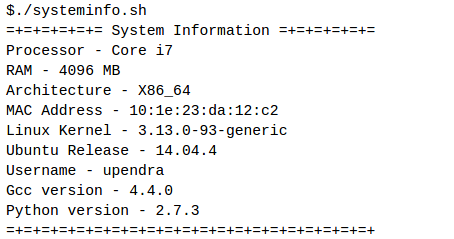
\includegraphics[scale=0.7]{images/Selection_001}	
	\end{figure}
	\subsection{Assumptions}
	The output is to be processed in the exact manner as shown in the image
	\pagebreak
	\subsection{Structure Chart}
	\begin{figure}[h!]
	\centering
	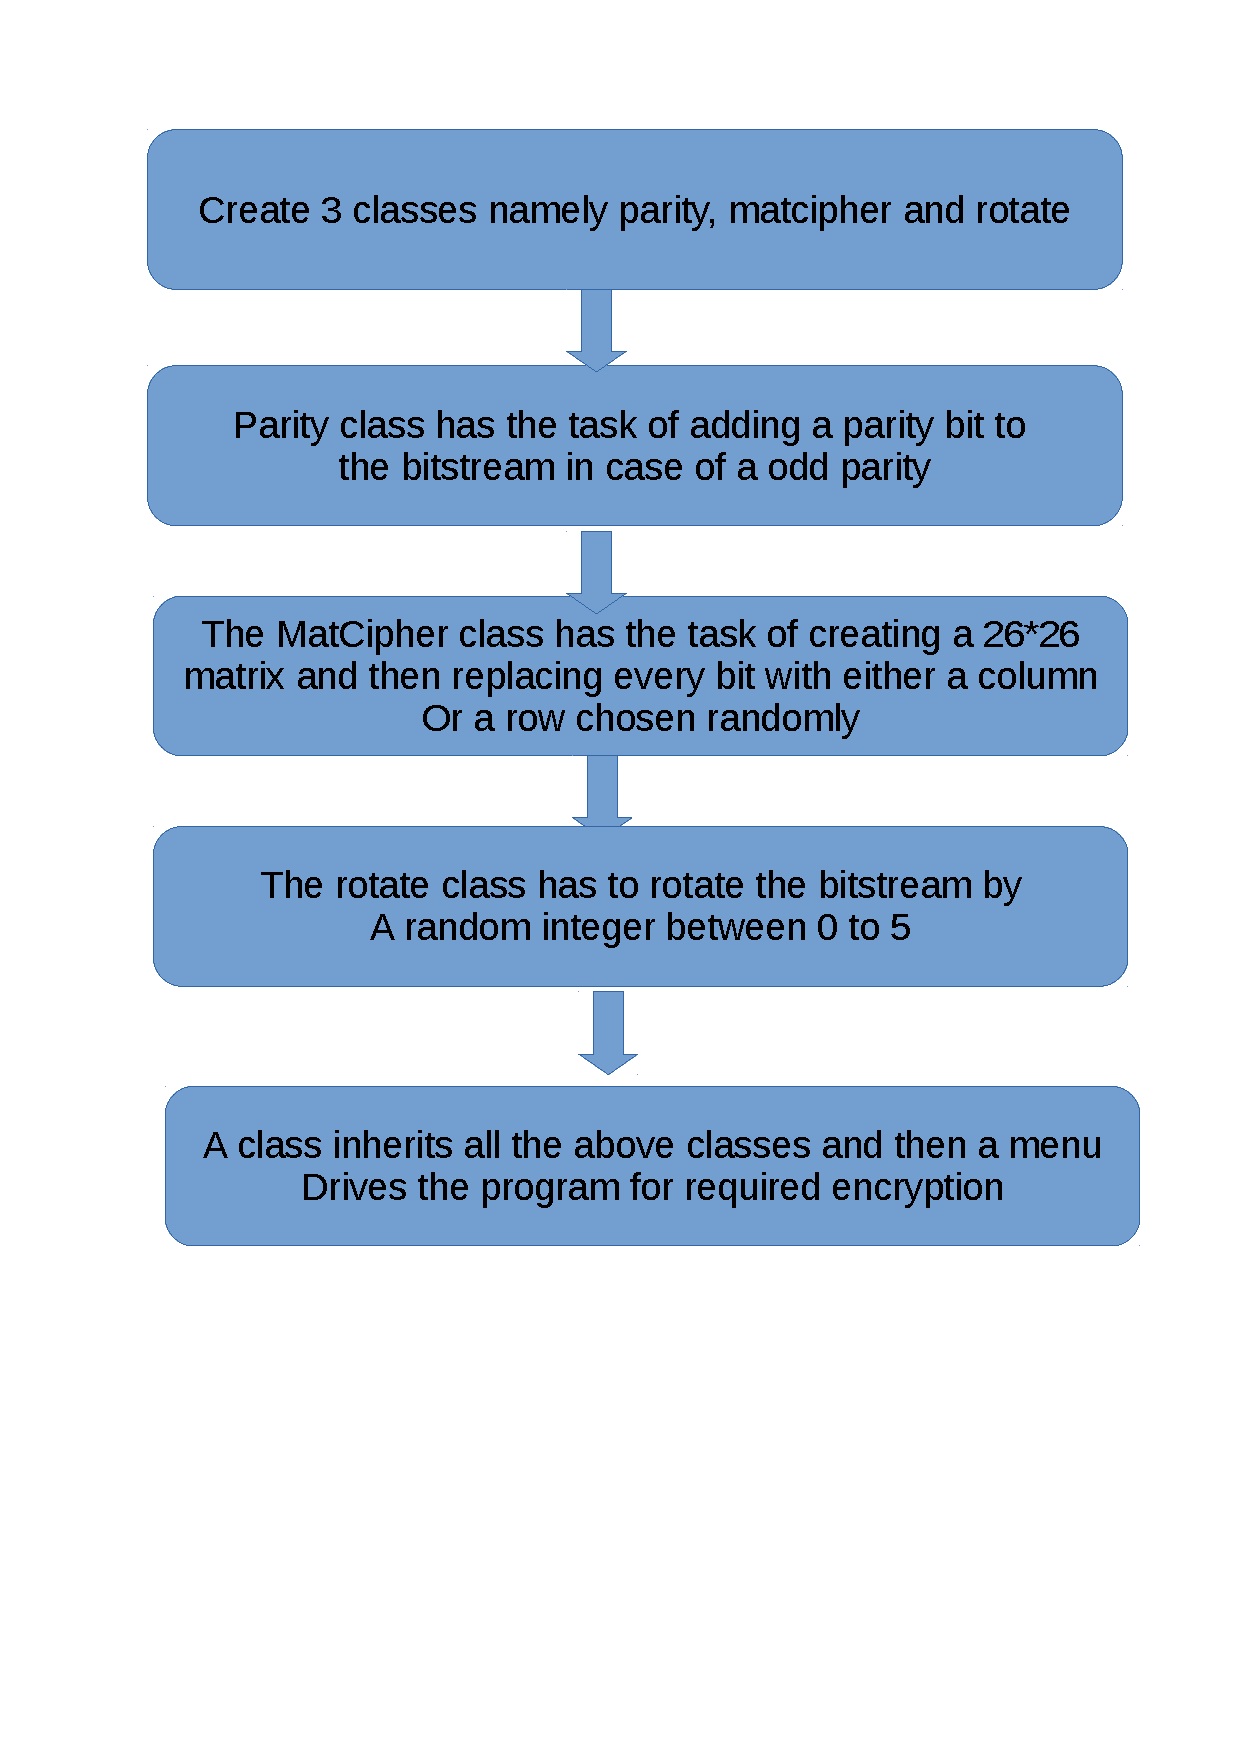
\includegraphics[scale=0.7]{images/shots22}
	\caption{Structure chart for problem 2}	
	\end{figure}
	\pagebreak
	\subsection{Screenshots}
	\begin{figure}[h!]
	\centering
	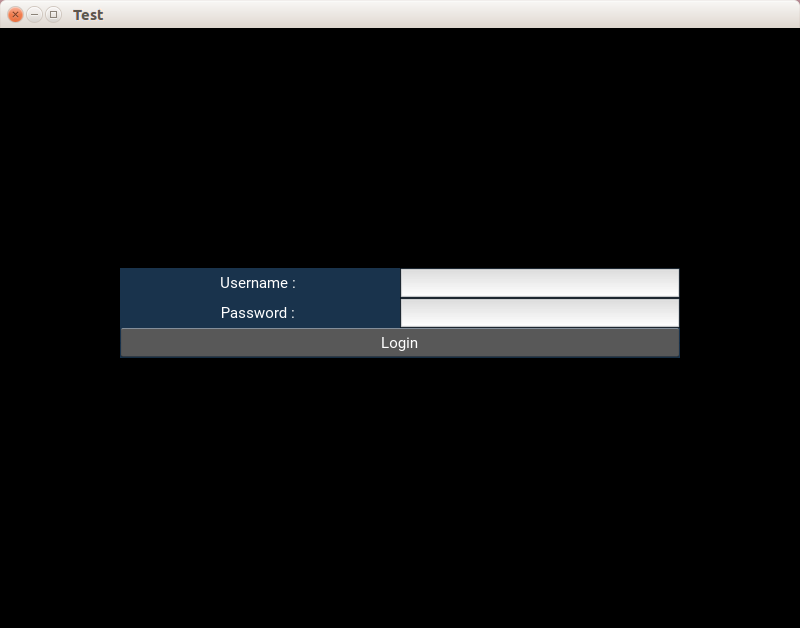
\includegraphics[scale=0.8, center]{images/screenshot2}
	\caption{Screenshot for problem statement 2}
	\end{figure}
	\pagebreak
\section{Problem Statement 3}
\textbf{Part - 1 -}\\
Write shell script to emulate behaviour of bash, but also record every command put up on terminal on a logger.txt file along with time stamp. Your command prompt should look like normal bash command prompt. \\
	\subsection{Assumptions}
	The output is to be processed in the exact manner as shown in the image\\
	\begin{figure}[h!]
	\centering
	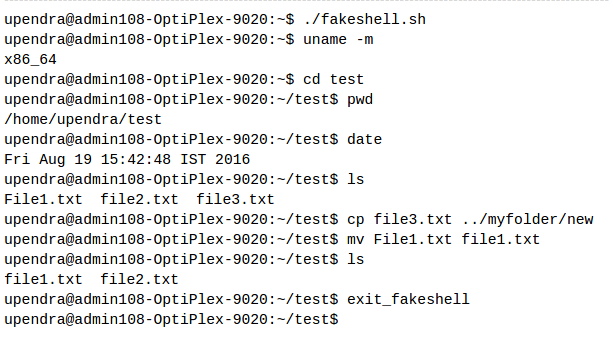
\includegraphics[scale=0.7]{images/Selection_004}	
	\end{figure}
	\pagebreak
	\subsection{Structure Chart}
	\begin{figure}[h!]
	\centering
	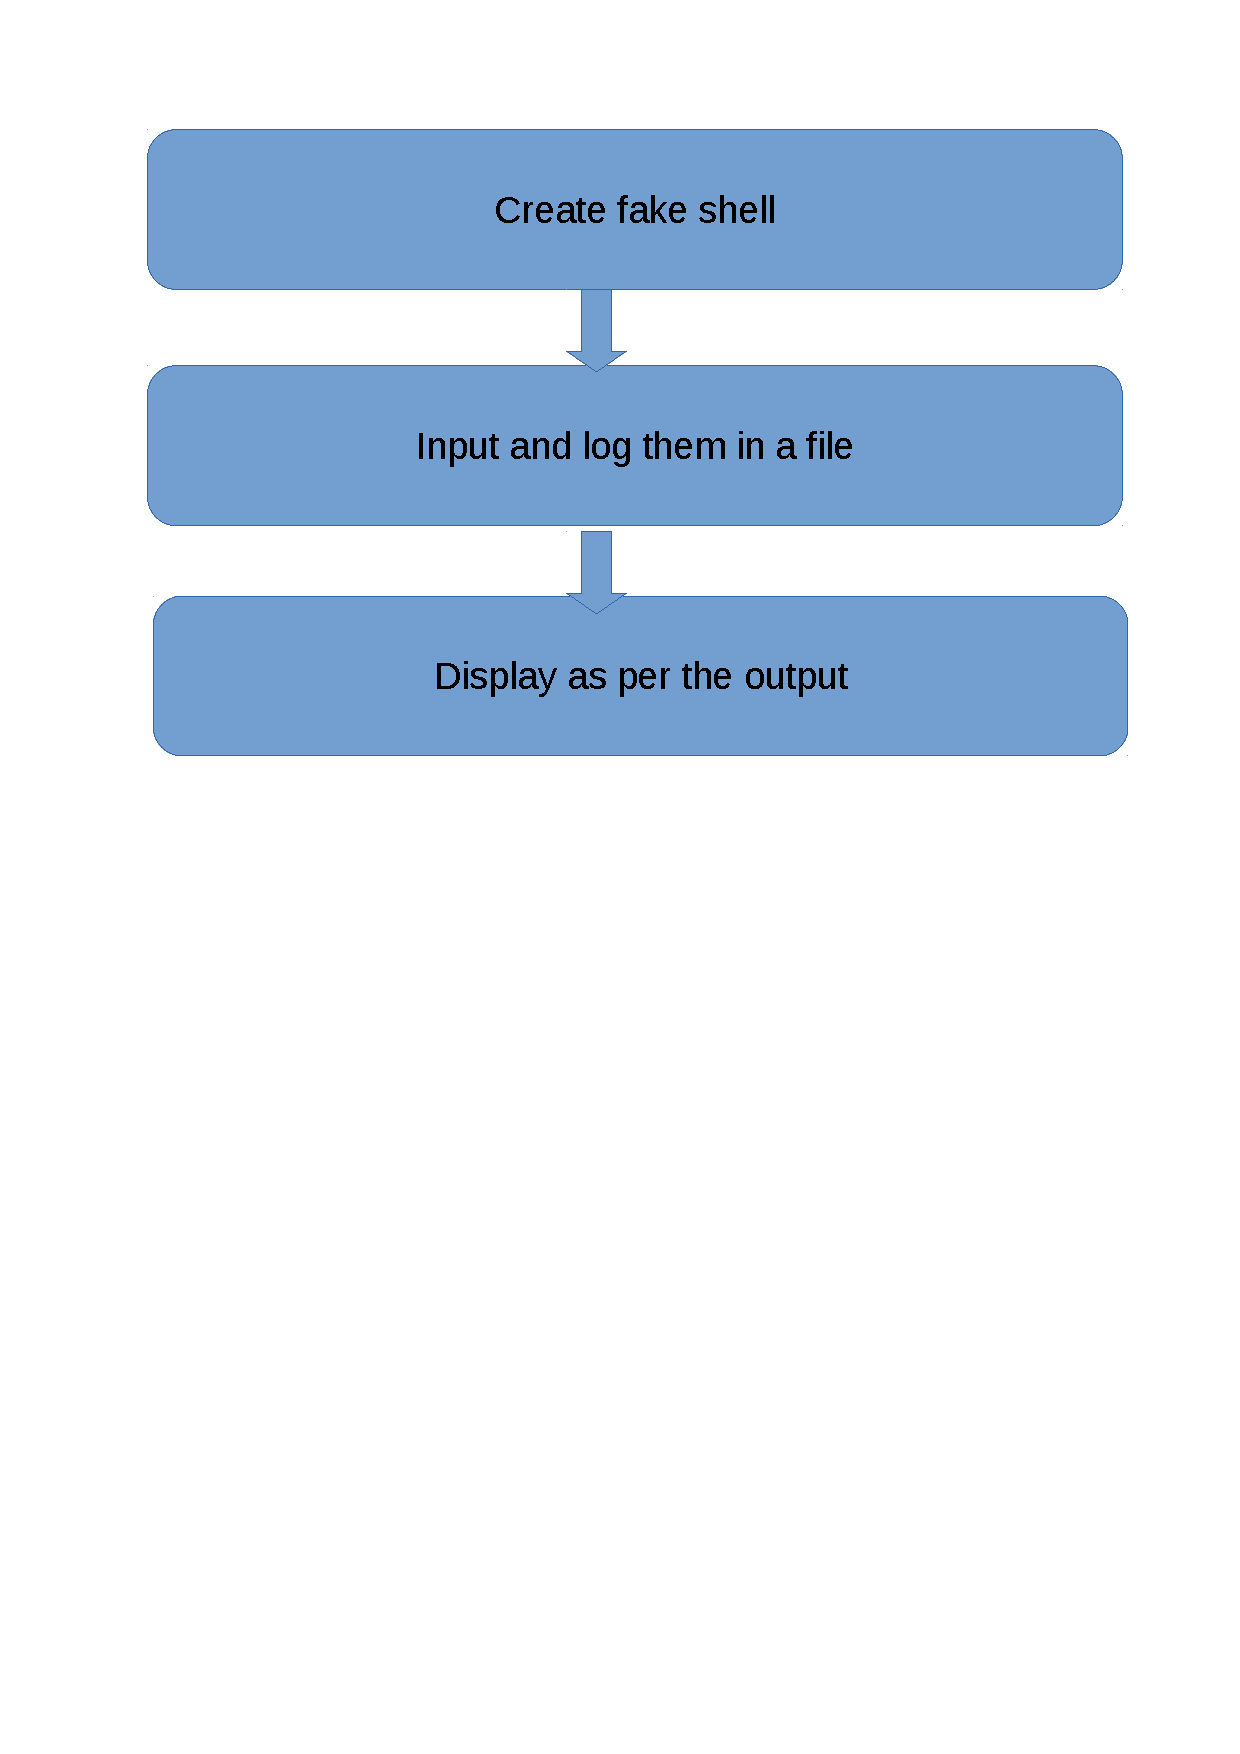
\includegraphics[scale=0.7]{images/shots33}
	\caption{Structure chart for problem 3}	
	\end{figure}
	\pagebreak
	\fi
	\pagebreak
\section{Epilogue}
The execution of the first problem involved me to break it down and then try to figure out solution to each and every part of it. To some extent I feel I have been successful in justifying the problem.\\
Whereas for problem statement 2, it was a different but not so difficult problem statement compared to problem 1. \\
Then i found the problem 3 to be the toughest of all problems.\\
This week's assignment too has taught me a lot of things on which I shall further improve upon in the next assignment.\\
\bibliography{biblio}
\bibliographystyle{ieeetr}
\nocite{*}
\end{document}